% This chapter will serve as an introduction to dark-matter physics

\chapter{Introduction}
	\label{chap:IntroChapter}

	\section{Neutrinos and neutrinoless double-beta decay ($\nonubb$)}
	
	Neutrinos are blah blah Wolfgang.  
	
	  Neutrino oscillation experiments have shown that neutrinos are massive but
cannot determine the absolute neutrino mass scale or the nature of the neutrino
mass (see, e.g.~\cite{Mes04}).  Neutrinoless double-beta decay ($\nonubb$) is a
process which, if discovered, would imply that the neutrino is its own
antiparticle (a so-called `Majorana' particle) and would define the neutrino
mass scale.  $\nonubb$ could occur in several even-even nuclei (e.g.~$^{48}$Ca,
$^{76}$Ge, $^{130}$Te, $^{136}$Xe, etc.) otherwise stable against
single-beta decay and is characterized by the emission of two electrons with
total kinetic energy equal to the Q-value of the reaction.  For example:
\begin{equation}
(Z,A) \rightarrow (Z+2,A) + e^- + e^-
\end{equation} 

where the Q-value is the mass difference $M(Z,A)-M(Z+2,A)-2m_e$.
A schematic of a possible lepton-number-violating mechanism for neutrinoless double-beta
decay is shown in Figure~\ref{fig:DBDK}.  Assuming left-handed currents and
that the decay is dominated by the exchange of a light massive Majorana
particle, the half-life of $\nonubb$ can be related to the effective mass of
the neutrino by:

\begin{equation}
\left( T_{1/2}^{0\nu}\right)^{-1} = G^{0\nu} |M^{0\nu}|^2 \langle m_{\nu_{\beta\beta}} \rangle^2  
\end{equation} 

where $G^{0\nu}$ refers to an exactly calculable phase-space integral, 
$|M^{0\nu}|^2$ is a nuclear matrix element, and $\langle m_{\nu{\beta\beta}}\rangle$
is the effective neutrino mass.  $^{76}$Ge currently holds the best limit for
the $\nonubb$ half-life: $T^{0\nu}_{1/2}\geq 1.6\times10^{25}$~\cite{Bau99}.
Several review articles exist outlining the current theoretical and
experimental landscape (see e.g.~\cite{Ell02,Bara07}).  
Two-neutrino double-beta decay ($\twonubb$) is a related 
decay that can exist in the same nuclei allowed to undergo $\nonubb$:  

\begin{equation}
(Z,A) \rightarrow (Z+2,A) + e^- + e^- + \bar{\nu}_e + \bar{\nu}_e
\end{equation}

The $\twonubb$ process has been seen in several nuclei including $^{76}$Ge and has
a half-life for these nuclei around $T^{2\nu}_{1/2}\sim10^{20}$~yrs.  

		\begin{figure}
			\centering
			\def\figheight{0.4\textheight}
			 \subfigure[$\twonubb$] {
			 	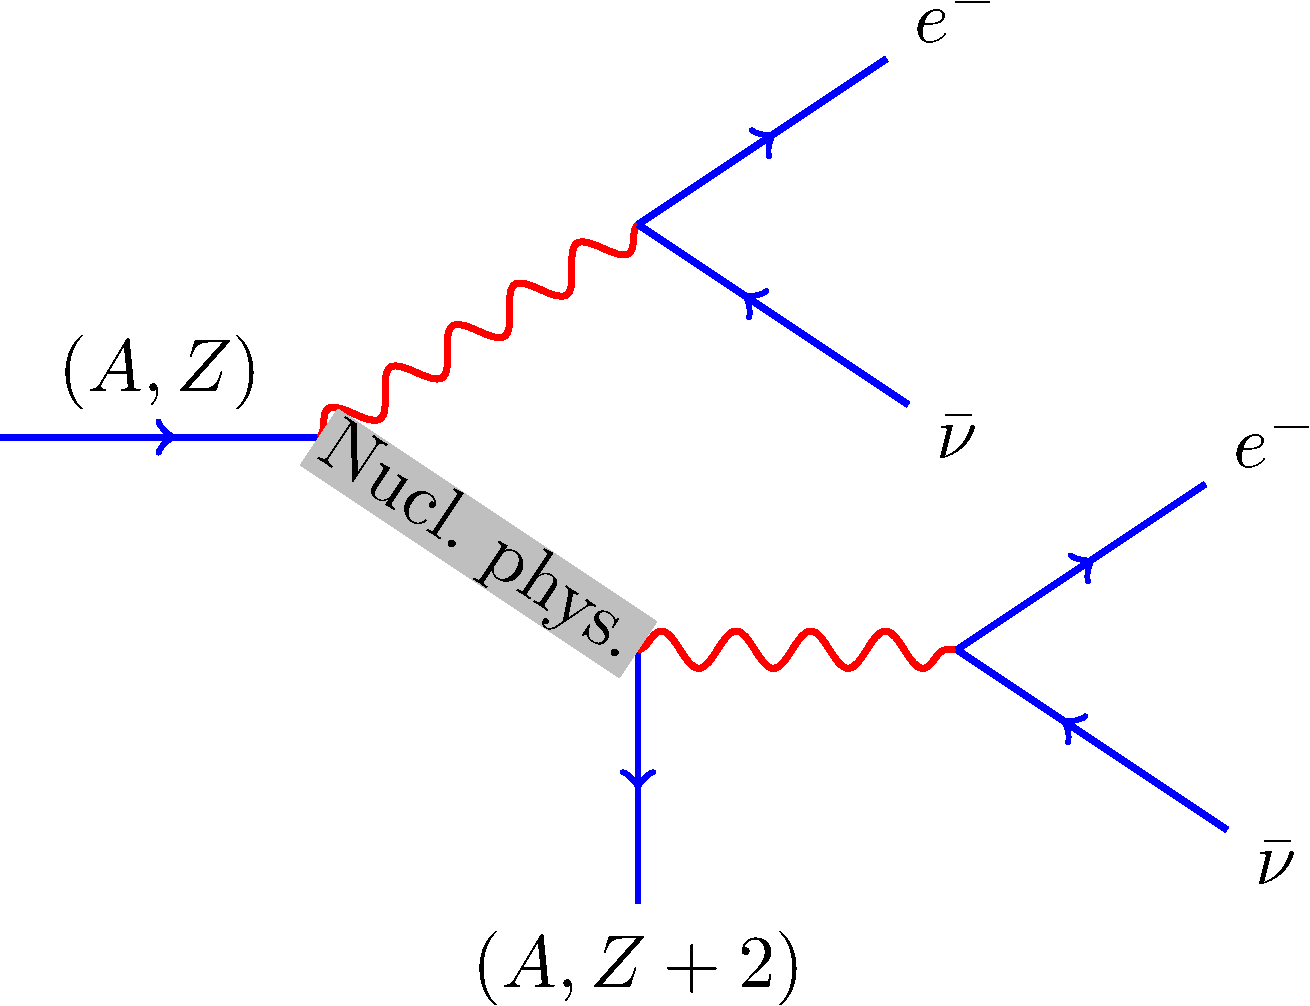
\includegraphics[height=\figheight]{2nubbDecay}
			}
			\subfigure[$\nonubb$]{
				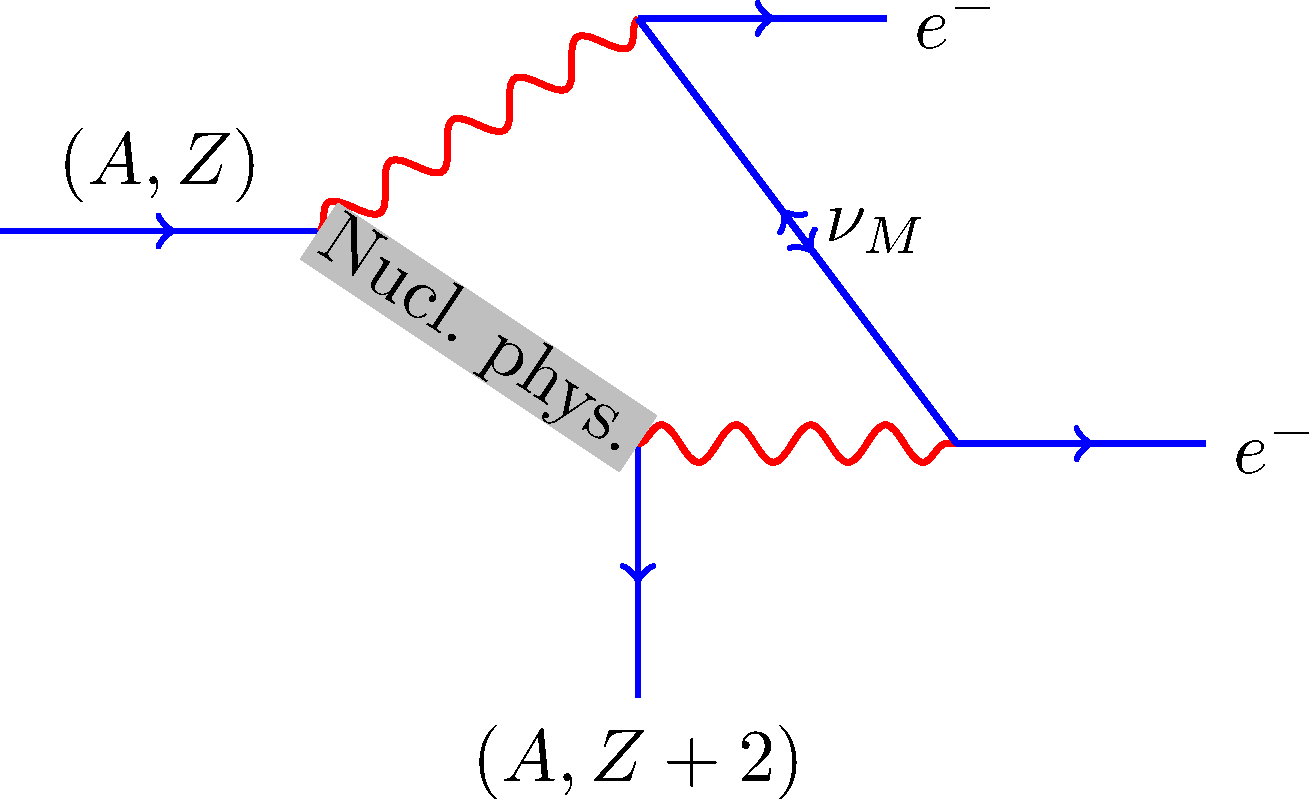
\includegraphics[height=\figheight]{0nubbDecay}
			}
		\caption{Schematic figure of the two types of double-beta decay, the 2$\nu$ mode and the 0$\nu$ mode.  
			In this schematic, the 0$\nu$ mode is mediated through the exchange of a virtual Majorana neutrino, $\nu_{M}$.}
		\label{fig:DBDK}
		\end{figure}
 

	
	\section{The \MJ\ experiment}
	\label{sec:MJExperiment}
	
The search for a rare process such as $\nonubb$ necessarily involves maximizing the magnitude of the expected signal while
simultaneously reducing backgrounds that may mimic the sought-after process.  
The \MJ~experiment proposes to search for $\nonubb$ in \gersevensix~using high-purity
germanium as both source and detector, thereby maximizing a possible signal from $\nonubb$. 
The first stage of this experiment will involve the deployment of 20-40~kg of germanium in a arrayed fashion in a \minmod~module with the goal to determine
the feasibility of scaling up to the 1-tonne scale.  To achieve this, the \MJ~experiment seeks to demonstrate less than
1~background count per year per tonne of enriched material in the
region-of-interest, a $\sim4$~keV window around the $\beta\beta$-decay
Q-value of $^{76}$Ge (2039~keV).  A low-capacitance, low-noise p-type point contact (\ppc)
detector will be deployed in these modules to take advantage of characteristics which make 
them beneficial for rare-process searches in general and for looking for $\nonubb$ in particular.  These characteristics and other details about \ppc~detectors will be discussed in Section~\ref{sec:PPCDets}.  

To achieve its background goals, the \MJ~experiment will employ standard techniques for background reduction including: creation of detector mounts, cryostats, and other components close to the detectors out of ultra-clean electroformed copper and other radiopure materials; use of passive shielding against external radiation including a lead shield for gamma radiation and a borated polyethylene shield for the moderation of cosmic-ray-induced neutrons; use of active shielding (vetos) against cosmic-ray muons; and deployment of the module underground in the Deep Underground Science and Engineering Lab (DUSEL) at Homestake, South Dakota, for moderation of cosmic-ray muons.  Engineering drawings given in Figures~\ref{fig:MJEngDrawing1} and~\ref{fig:MJEngDrawing2}shows both the cryostat design and the expected shield construction, and indicates the modular design of the experiment; additional, independent cryostats may be deployed within the same shield geometry.  The expected sensitivity of this first stage, 
assuming 3 years with 30~kg of enriched material or 90~kg-yr of $^{76}$Ge
exposure, is T$_{1/2}\geq 10^{26}$.  Further information on the
\MJ~experiment can be found in technical documents \footnote{Available:
http://majorana.npl.washington.edu/general.php}. 

	
		\begin{sidewaysfigure}
			\centering		
			\def\figheight{0.45\textheight}
			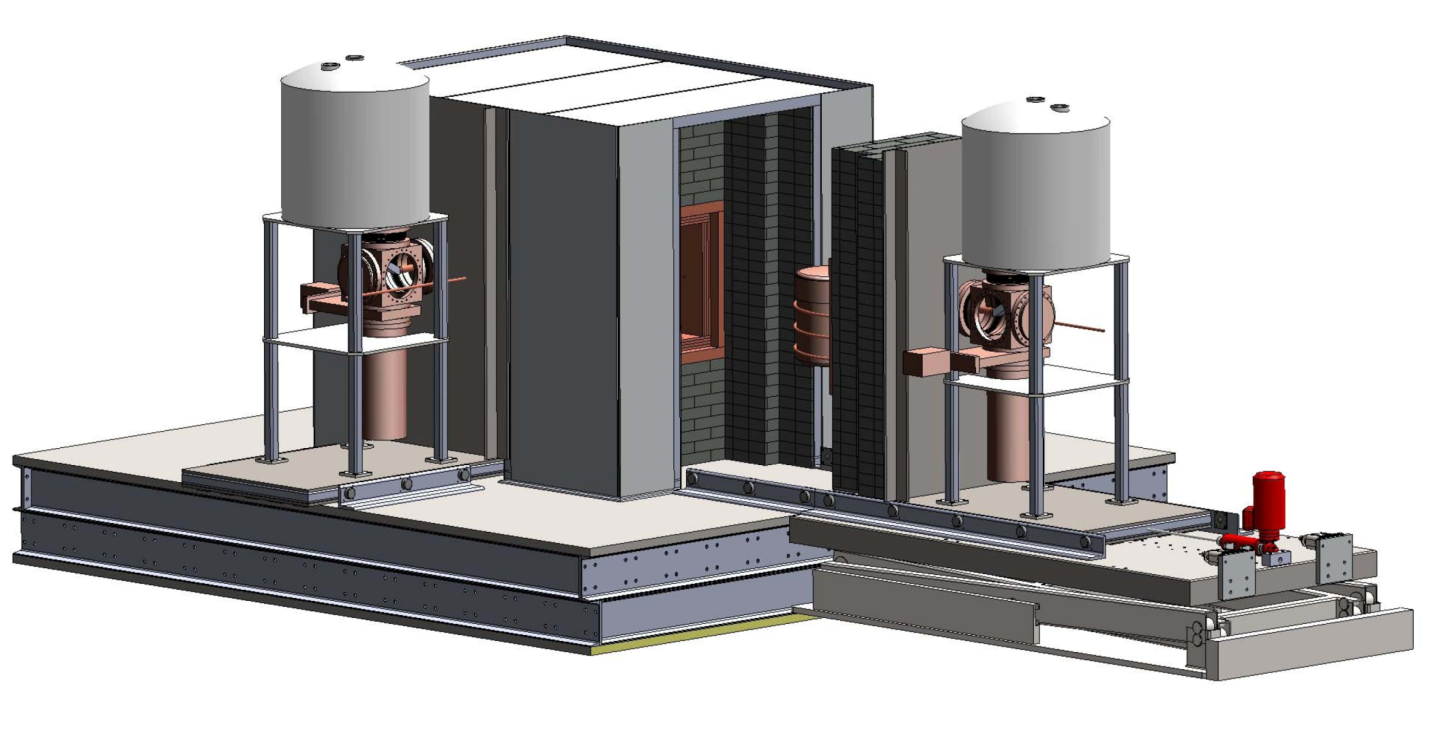
\includegraphics[height=\figheight]{ShieldDesign}
			\caption[\MJ~\minmod~shield geometry]{\MJ~\minmod~shield geometry.  The modular design of the shield will 
			enable a phased deployment of cryostats, allowing detectors to be easily added after commission of the experiment.}
			\label{fig:MJEngDrawing2}
		\end{sidewaysfigure}
	
		\begin{figure}
			\centering		
			\def\figheight{0.45\textheight}
			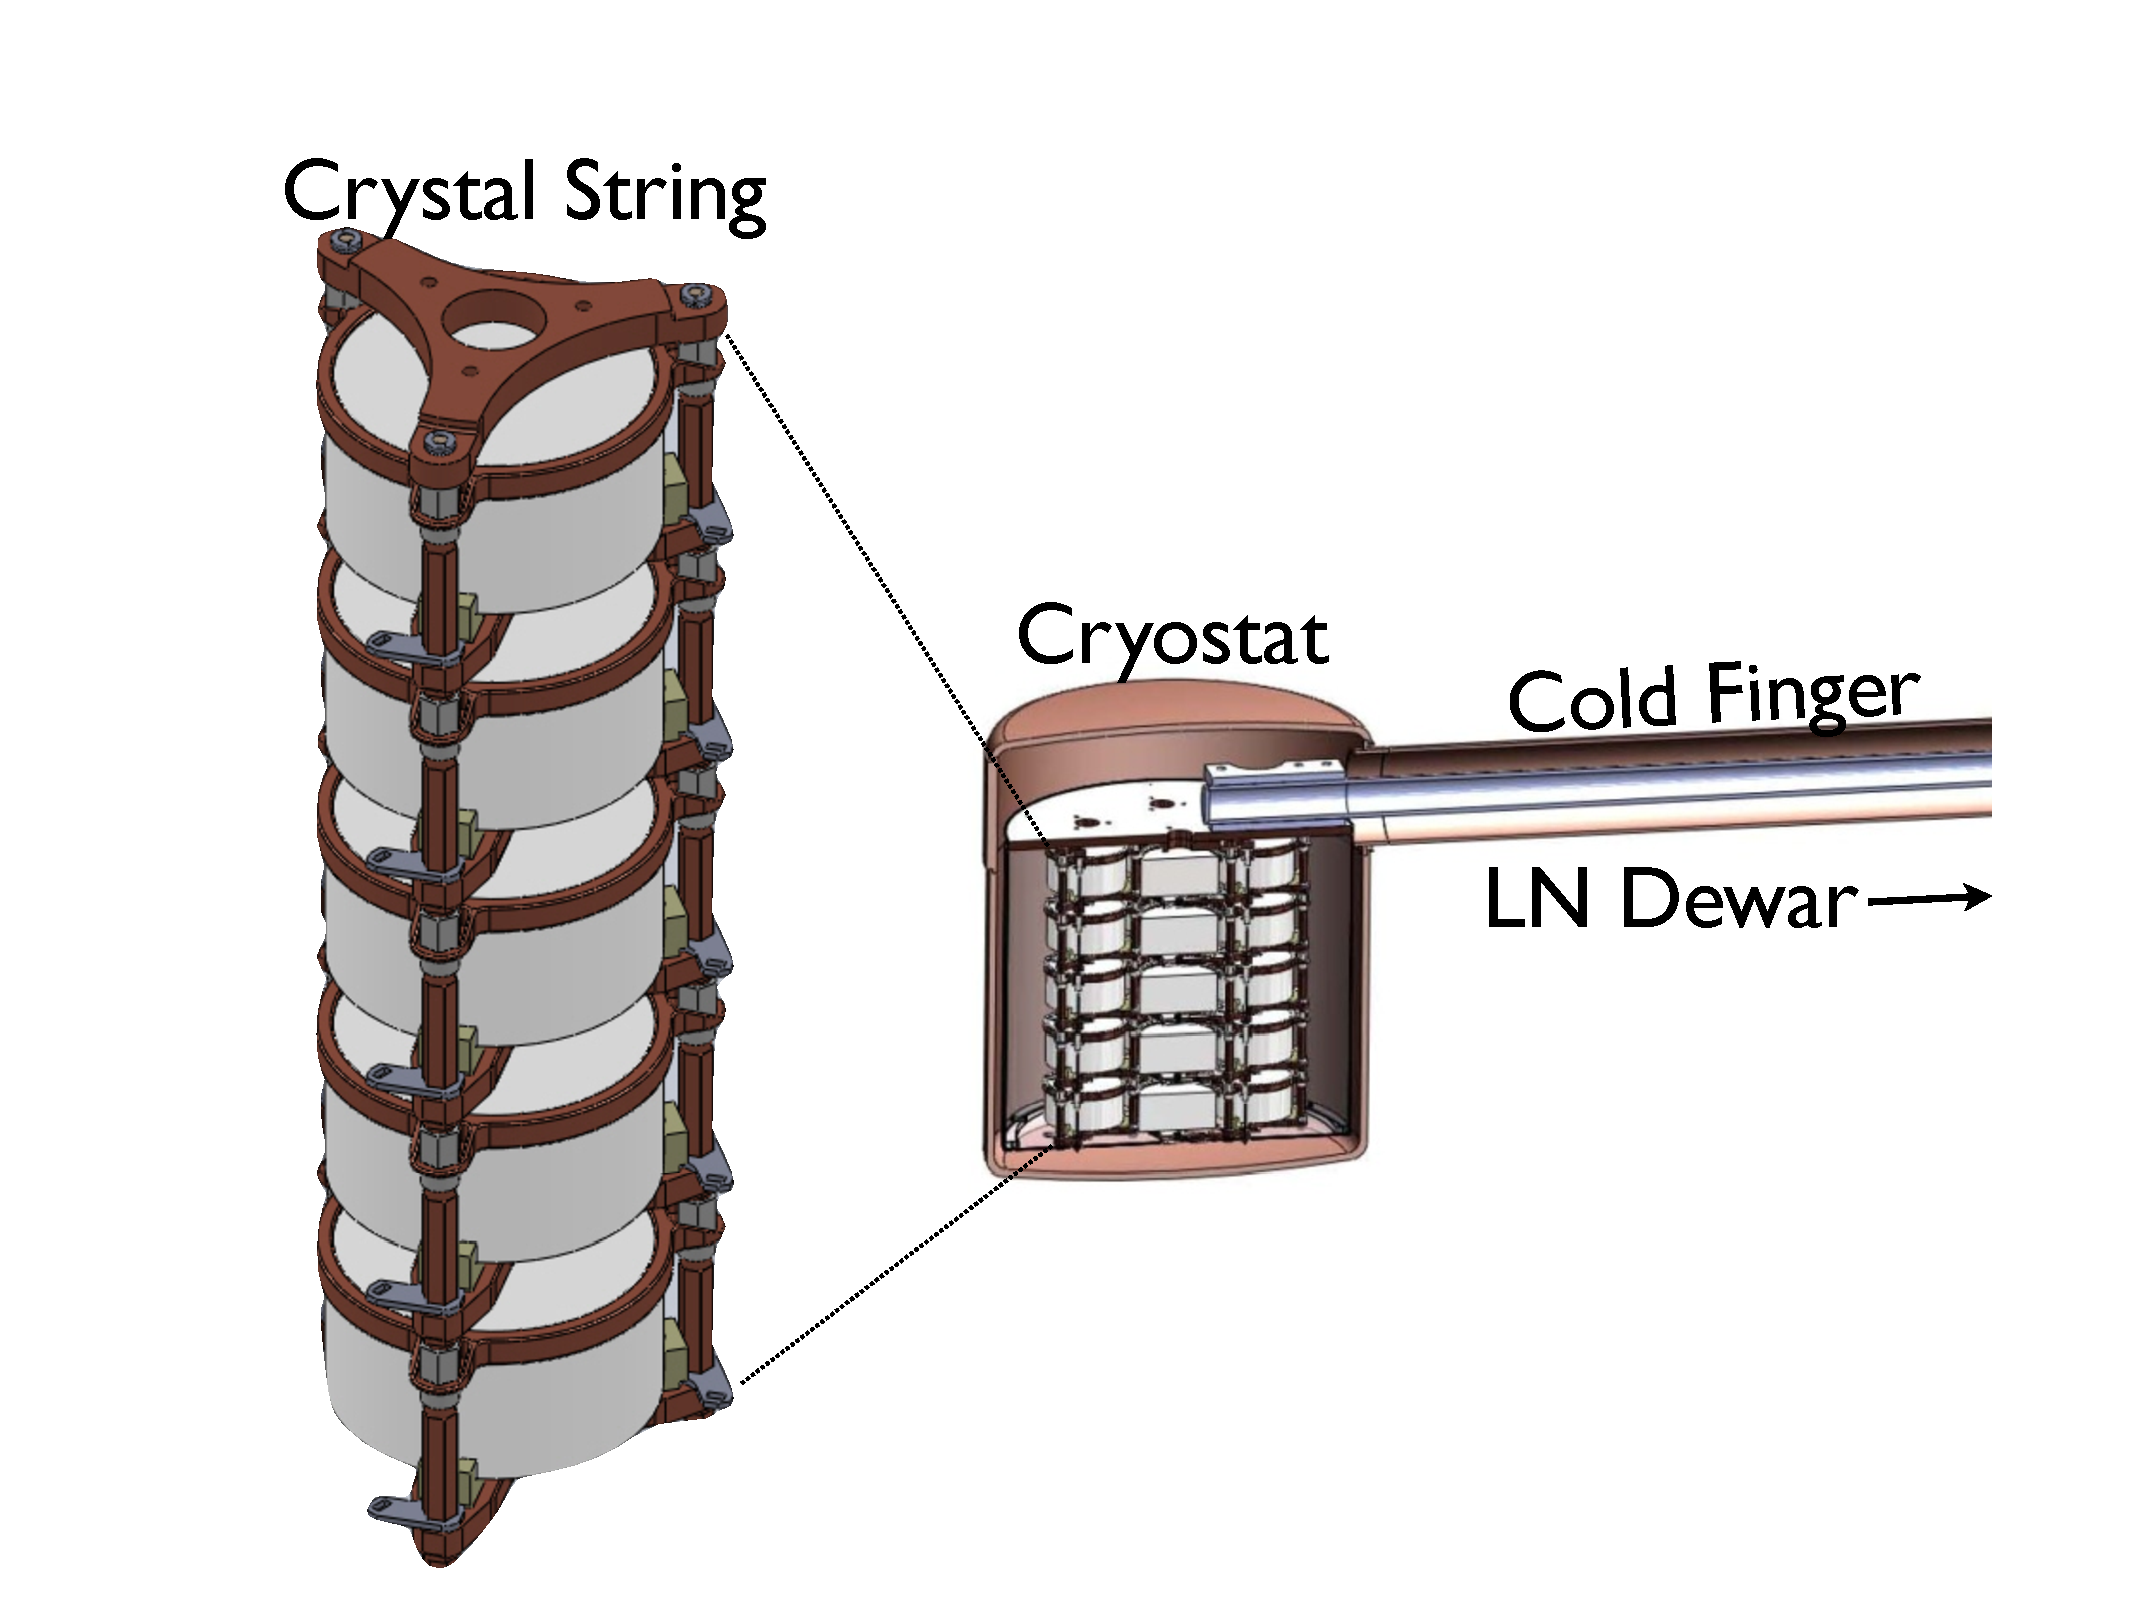
\includegraphics[width=0.9\textwidth]{CrystalCryostatDesign}
			\caption[\MJ~\minmod~cryostat and crystal string geometry]{\MJ~\minmod~cryostat and crystal string geometry, the
			crystal string houses .}
			\label{fig:MJEngDrawing1}
		\end{figure}

	
	\section{P-type point contact (\ppc) germanium detectors}
	\label{sec:PPCDets}

  P-type point-contact (\ppc) germanium detectors are an exciting detector
technology whose characteristics provide powerful tools in the search for
$\nonubb$ and enable searches for other rare physics processes at low energy, e.g.~dark matter.  
The electrode geometry of \ppc~detectors significantly reduces the
capacitance, reducing the energy threshold and enhancing the detector's
ability to detect low-energy ($\sim100$~eV) processes.  Figure~\ref{fig:PPCGeom} shows a picture of the geometry of this detector in comparison to a standard semi-coaxial crystal.  In addition to improving the electronic response of the detector, the crystal geometry also yields a weighting field strongly peaked at the readout electrode.  This means that as charge drifts to the p contact after being created from energy deposition in the crystal (e.g.~from a physics interaction), no signal will be induced in the contact until the drifting charge is very near ($\sim2$~cm) the contact.  Additionally, charge drift times are increased by the longer drift paths.  These two characteristics coupled together improve the ability to distinguish between charge originating from one point in the crystal or from multiple sites in the detector.

An n-type detector with a point-contact geometry was developed by Luke et
al.~in 1989, demonstrating detector capacitance on the order of
1~pF~\cite{Luke89}.  With such a low capacitance and therefore low energy
threshold this detector was seen as a potential tool for dark matter detection, but this detector 
exhibited poor energy resolution due to incomplete charge collection attributed to charge-trapping effects.  
		\begin{figure}
			\centering
			\subfigure[Point-contact geometry.]{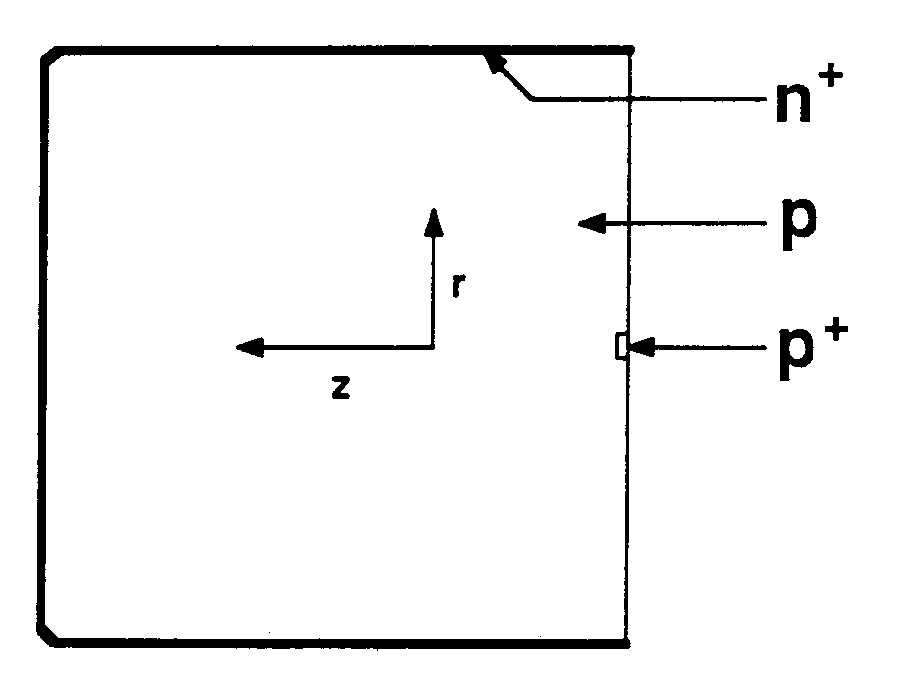
\includegraphics[height=0.2\textheight]{LukePPC}}
			\subfigure[Semi-coaxial geometry.]{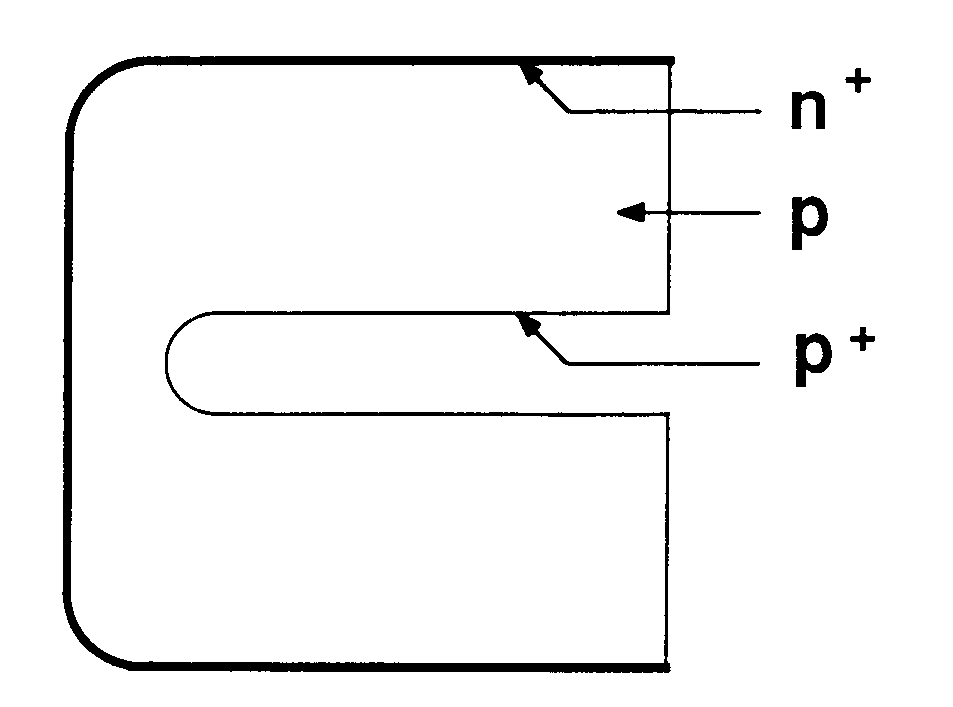
\includegraphics[height=0.2\textheight]{LukeCoax}}
			\caption[\ppc~detector geometry]{The left figure depicts the point-contact geometry, the right figure a conventional 
			         semi-coaxial geometry.  Figure adapted from~\cite{Luke89}.  The small diameter of the p contact in the
			          \ppc~detector reduces the capacitance of the detector improving the intrinsic noise characteristics.}
			\label{fig:PPCGeom}
		\end{figure}
  In 2007, Barbeau et al.~presented a new detector with a point-contact 
geometry which departed from previous convention in that it was made
of p-type instead of n-type material~\cite{Barb07}.  The reason for this
change was to take advantage of reduced sensitivity of p-type crystals to electron trapping in germanium.  
Because p-type crystals collect holes instead of electrons at the p contact of the crystal, they are less likely to 
see a degradation of signal from electron trapping~\cite{Hull:2005p2207}.
With these changes, Barbeau et al.~demonstrated
a resolution comparable to conventional semi-coaxial germanium detectors and
an energy threshold of 330~eV making them an excellent candidate for double-beta decay searches.  
Other work with these detectors has supported these conclusions (see e.g.~\cite{Hull:2008p2206,Aalseth:2008aa}).
%Additionally, using a collimated $^{241}$Am gamma source (59.5~keV), they demonstrated differences in pulse rise-times based upon position of interaction (see Figure~\ref{fig:MeasPulses}).   

%\begin{figure}
%\begin{center}
%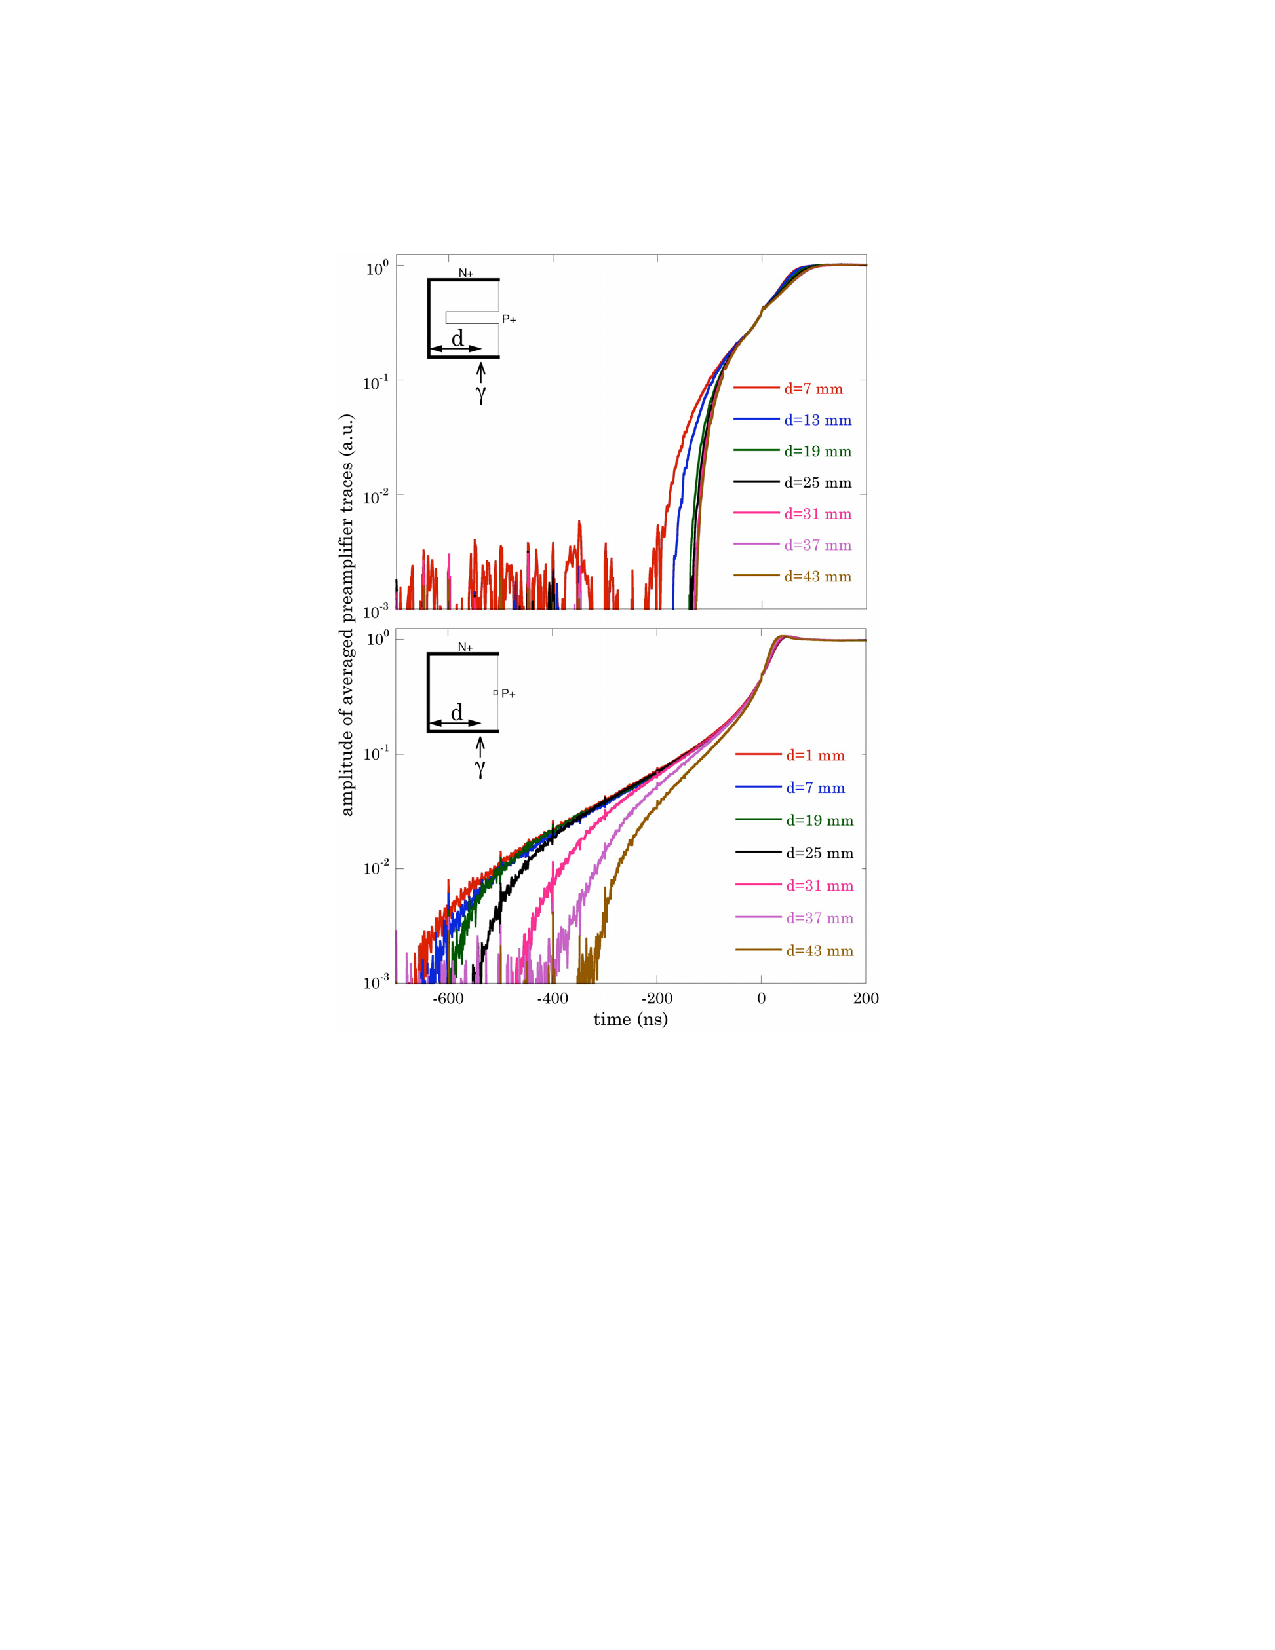
\includegraphics[width=0.8\textwidth]{BarbPPC}
%\caption{Pulses from a collimated ${241}$Am gamma source incident upon the surface
%         of a conventional semi-coax detector (top) and a p-type point-contact (bottom).
%         The expansion of the charge collection time in the \ppc~detector versus
%         the conventional semi-coax detector is evident.  (Figure from~\cite{Barb07}.)}
%\label{fig:MeasPulses}
%\end{center}
%\end{figure}

	\section{\ppc~detectors for the \MJ~experiment}

For the proposed \MJ~experiment, the characteristics of the \ppc~detector
will aid in the reduction of backgrounds and in enhancing the physics reach of
the experiment.  Since $\nonubb$ is an inherently single-site event, cutting out
multi-site events during data analysis provides a powerful background reduction
tool.  For conventional semi-coaxial detectors, various tools have been developed
to tag multi-site events based upon the shape of the measured pulse (see,
e.g.~\cite{Aal00}).  The expansion in time
of charge collection in \ppc~detectors makes distinguishing multi-site events easier and improves the efficiency for single-site acceptance vs. multi-site rejection of a pulse-shape analysis routine (see~\cite{Budjas:2009zu,Ren10}.

To improve the bandwidth of the detector readout it is necessary to
place front-end preamplification electronics (e.g.~field-effect transistors) nearby the detectors
inside the detector cryostat.  As with any low-background 
experiment the increase of material (and especially material close to
sensitive detectors) introduces potential radioactivity that could
increase background.  The single-contact nature of the \ppc~requires only one
front-end per crystal, thus reducing the material inside the cryostat and possibly
softening radiopurity requirements.

Cosmogenically-produced $^{68}$Ge is a significant background
source for the \MJ~experiment, decaying first via electron capture to $^{68}$Ga
(T$_{1/2}=271$~d) and then to $^{68}$Zn (Q=2921~keV, T$_{1/2}=68$~m).  The
initial decay is followed by the emission of Auger electrons and/or soft x-rays
from $\sim1.3$~keV to $\sim10.3$~keV, and it is possible to use these to tag
the $^{68}$Ge decay.  A time cut can then be introduced to veto events
occurring within a few $^{68}$Ga lifetimes to mitigate background from that
decay without seriously affecting detector live time.   \ppc~detectors have an
improved sensitivity to low-energy physics because of their low noise and 
low-energy threshold and so could significantly enhance the tagging of the
$^{68}$Ge decay.  This low-energy threshold will also
expand the physics reach of the \MJ~experiment, making it sensitive to
low-energy nuclear recoils and enhancing its capacity as a dark matter
detector.  This is a question considered in much more detail 
throughout the remainder of this dissertation.


%The low energy threshold and low noise of the \ppc~detector won't necessarily
%improve a search for $\nonubb$ since the region-of-interest for $^{76}$Ge is at
%2039~keV, well above the energy region where electronic noise and detector
%capacitance dominate the overall noise.  

%An additional advantage of the \ppc~detectors, as with other p-type
%detectors, is its thick outer Li contact which tends to be on the order of
%$\sim0.5$~mm.  Alpha particles emitted from Rn daughters contaminating the
%surface of cryostat components in the \MJ~demonstrator module might provide
%a significant background source (see e.g.~\cite{Joh07}).  However, the outer
%Li contact of a p-type detector renders much of the outer surface insensitive
%to these decays.  Additionally, the outer contact improves the robustness of
%the surface making the detector less susceptible to damage during
%handling.  This is an important consideration especially for detectors 
%designed to be installed in an arrayed fashion.  

	\section{Searching for dark matter: low-energy physics with \ppc~detectors}
	
	% Galactic rotationl curves
	
	From cosmological observation there exists significant evidence that the matter density of the universe is mostly composed of non-luminous gravitationally-interacting particles referred to as `Dark Matter'.  Perhaps the most convincing empirical indications arise from measurements of galactic rotational curves.  To explain simply, astronomers measure the rotational velocity of stars in galaxies and determine the relation of this velocity versus the radial distance from galactic center.  One can compare this to the ex
An example of such a curve has been include from Reference~\cite{Begeman:1991iy} in Figure~\ref{fig:DMRotCurve}.

		\begin{figure}
			\centering
			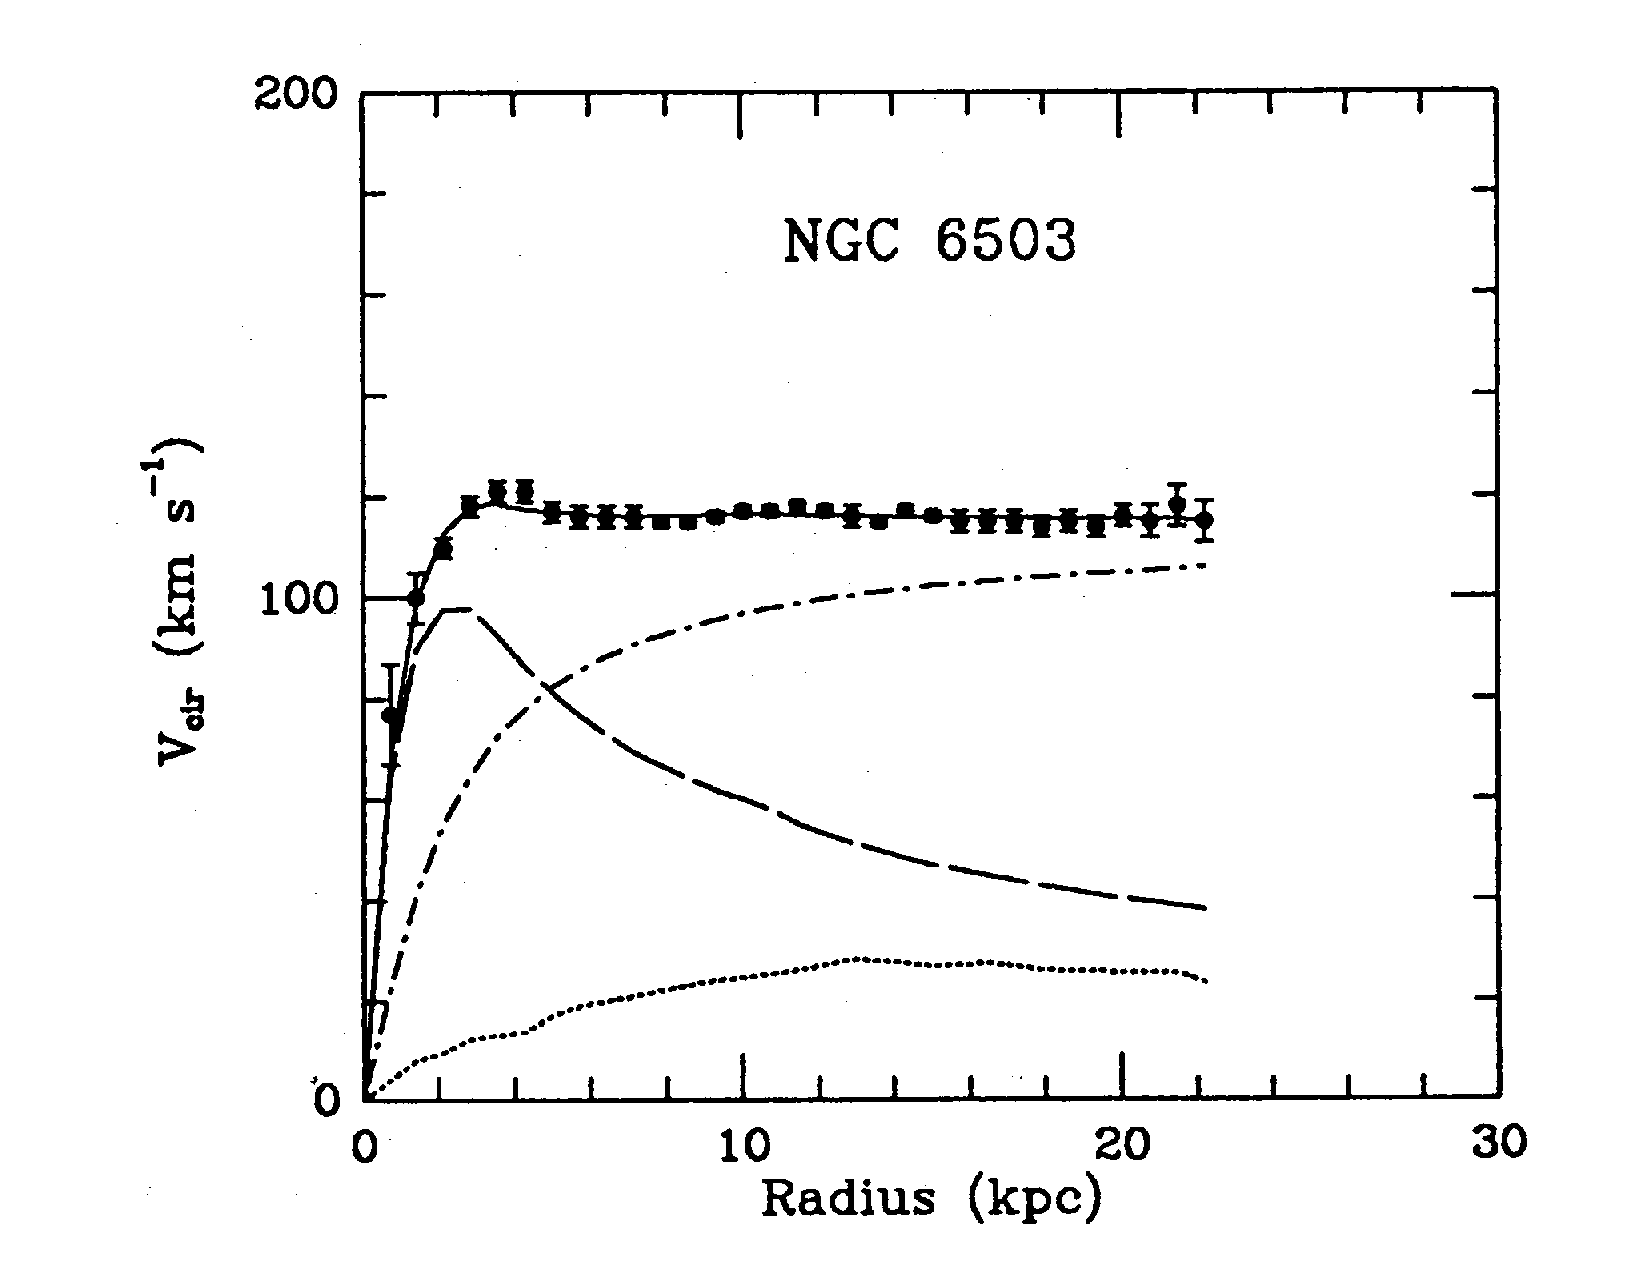
\includegraphics[width=0.9\textwidth]{DMRotationalCurves}
			\caption[Example galactic rotational velocity curve.]{Example galactic rotational velocity curve 
			from~\cite{Begeman:1991iy}.}
			\label{fig:DMRotCurve}
		\end{figure}
	% WMAP results (large-scale structure)
	
Though the primary purpose of the \MJ~experiment remains the search for $\nonubb$, the choice of detector technology for the experiment will enable sensitivity to other physics processes in low-energy regions.  

	% Bullet cluster
	% Dark matter candidates	
	
	\section{Outline of this dissertation}
